\begin{frame}[t]
    \begin{theorem}[P.Hall, 1935]
        В двудольном графе $G = \left( L, R, E \right) $ есть паросочетание, покрывающее долю $L$, если и только если:  $$\forall A \subset L: |A| \leq |N_G(A)|$$
    \end{theorem}
    
    \begin{proof}[Доказательство методом чередующихся путей]
        \renewcommand{\qedsymbol}{}
        \fbox{$ \Rightarrow $} Очевидно.
        
        \fbox{$ \Leftarrow $} Обсудим идею доказательства. Будем добавлять рёбра в паросочетание $M$ алгоритмом. Зная, что $\forall A \subset L: |A| \leq |N_G(A)|$, на шаге $k \leq n$ (пусть $|L| = n$) будем доказывать, что можно добавить ещё одну вершину в наше паросочетание. В итоге получим паросочетание, покрывающее $L$. Докажем это индукцией по шагам алгоритма.
    \end{proof}
\end{frame}

\begin{frame}[t]
    \small
    \underline{\textcolor{blue}{База: $k = 1$}}. Тогда выберем произвольную вершину и применим к ней условие Холла:  $|N_G (A)| \geq 1$. Значит, её можно соединить с какой-то вершиной из $R$.
    
    \underline{\textcolor{blue}{Переход}}. Выберем ещё не насыщенную паросочетанием $M$ вершину $v$, и рассмотрим все вершины, достижимые из неё (граф $G'$), при условиях:
     \begin{itemize}
        \item Из $L$ в $R$ можно ходить по любым рёбрам.
        \item Из $R$ в $L$ можно ходить \textit{только по рёбрам построенного ранее паросочетания}.
    \end{itemize}

    \begin{figure}[h]
        \centering
        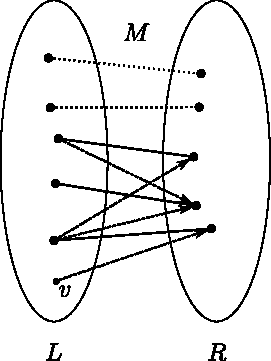
\includegraphics[width=0.3\textwidth]{images/condition}
    \end{figure}
    
\end{frame}

\begin{frame}[t]
    \begin{itemize}
        \item Очевидно, что $G'$ -- подграф графа $G$.
        \item Применим к нему условие Холла. Тогда вершин в  $R(G')$ не менее, чем в $L(G')$, откуда найдётся ещё хотя бы 1 вершина, с которой $G'$ связен. Обозначим её $u$.
    \end{itemize}

            \begin{figure}[h]
                \centering
                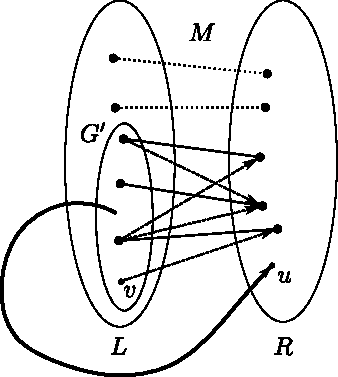
\includegraphics[width=0.4\textwidth]{images/connectivity_hall}
                \label{fig:connectivity_hall}
            \end{figure}
    
\end{frame}

\begin{frame}[t]
    \begin{itemize}
        \item Если $v \leadsto u$, то соединяем их и получаем требуемое. Иначе рассмотрим $vu$ путь, предварительно покрасив рёбра паросочетания \textcolor{blue}{синим}.
    \end{itemize}

    \begin{figure}[h]
        \centering
        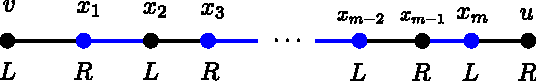
\includegraphics[width=0.8\textwidth]{images/longerway}
        \label{fig:longerway}
    \end{figure}

    \begin{itemize}
        \item Остаётся заметить, что $vu$-путь удлиняющий, а значит, если мы заменим паросочетание на паросочетание из чёрных рёбер, то, во-первых, оно останется паросочетанием, а во-вторых, мы насытим вершину $v$ и оставим насыщенными уже существовавшие вершины.
        \item Таким, образом, мы по индукции доказали, что при условии Холла можно добавить $|L|$ вершин в паросочетание $ \Rightarrow$ паросочетание $M$ покрыло $L$. 
            \hfill \qedsymbol{}
    \end{itemize}
\end{frame}
